%==============================================================================
% Exemplo de Trabalho Individual com a classe texufpel
%
% O tema é o mesmo do exemplo de exame de qualificação
% (qualificação/exemplo-qualificacao.tex): o roteamento da coleta seletiva de
% Pelotas com janelas de tempo. Aqui ele aparece como trabalho individual de
% doutorado, uma revisão da base teórica feita antes da qualificação. O texto
% de cada seção explica o recurso que aparece nela. As particularidades do
% trabalho individual estão marcadas com "TRABALHO INDIVIDUAL" nos
% comentários.
% Para começar o seu trabalho, copie este arquivo, troque os dados do
% preâmbulo (os comentários "ALTERE" indicam o que mudar) e substitua o texto
% dos capítulos.
%
% Compilação (a partir da pasta raiz do repositório, onde estão a classe, o
% estilo abnt.bst, o bibliografia.bib e a pasta imagens/):
%   pdflatex trabalho-individual/exemplo-ti
%   bibtex   exemplo-ti
%   pdflatex trabalho-individual/exemplo-ti
%   pdflatex trabalho-individual/exemplo-ti
% No Overleaf, basta marcar trabalho-individual/exemplo-ti.tex como documento
% principal.
%
% As páginas citadas nos comentários são as do Manual de normas UFPel para
% trabalhos acadêmicos (2023).
%==============================================================================

% Opções da classe:
%   tid  trabalho individual de doutorado; use ti para o de mestrado
% TRABALHO INDIVIDUAL: o trabalho não é depositado na biblioteca. A classe
% não gera capa (a opção capa é ignorada) nem a referência do trabalho acima
% do resumo e do abstract.
\documentclass[tid]{texufpel}

%------------------------------------------------------------------------------
% Pacotes usados neste exemplo. Nenhum é obrigatório: carregue só o que o seu
% trabalho usar. A classe já carrega graphicx, hyperref, natbib e caption.
%------------------------------------------------------------------------------
\usepackage{amsmath}        % equações alinhadas (align) e \eqref
\usepackage{pdfcomment}     % \pdftooltip: dica com o significado da sigla
\usepackage{array}          % colunas alinhadas à esquerda no quadro (L{...})

% Coluna de largura fixa com texto alinhado à esquerda, sem os espaços largos
% que a justificação cria em colunas estreitas.
\newcolumntype{L}[1]{>{\raggedright\arraybackslash}p{#1}}

%------------------------------------------------------------------------------
% Dados institucionais. ALTERE para o seu programa.
% \curso é a área do título: "Doutor em Ciência da Computação".
% Se a unidade for feminina (Faculdade, Escola), use \unidade[a]{...}.
%------------------------------------------------------------------------------
\unidade{Centro de Desenvolvimento Tecnológico}
\programa{Programa de Pós-Graduação em Computação}
\curso{Ciência da Computação}

%------------------------------------------------------------------------------
% Dados do trabalho. ALTERE.
% Os nomes abaixo são de grandes nomes da Computação e servem só de exemplo.
% Substitua pelos nomes da sua orientação.
%------------------------------------------------------------------------------
\title{Roteamento de veículos com janelas de tempo: fundamentos para a coleta seletiva urbana}

\author{Lovelace}{Ada}                          % ALTERE: autor(a)
\advisor[Prof.ª~Dr.ª]{Liskov}{Barbara}          % ALTERE: orientador(a)
\coadvisor[Prof.~Dr.]{Dijkstra}{Edsger W.}      % ALTERE: coorientador(a), opcional

% Ano da folha de rosto. Sem este comando, a classe usa o ano em que o
% documento é compilado. ALTERE.
\date{novembro}{2027}

% Palavras-chave: iniciais minúsculas (exceto nomes próprios), separadas por
% ponto e vírgula, a última terminada em ponto (Manual, p. 15).
\keyword{coleta seletiva;}
\keyword{heurísticas;}
\keyword{janelas de tempo;}
\keyword{problema de roteamento de veículos.}

\keywordeng{selective waste collection;}
\keywordeng{heuristics;}
\keywordeng{time windows;}
\keywordeng{vehicle routing problem.}

\begin{document}

% Orientadora ou coorientadora: troque o rótulo.
\renewcommand{\advisorname}{Orientadora}

\maketitle   % folha de rosto (sem capa, por ser trabalho individual)

% TRABALHO INDIVIDUAL: sem ficha catalográfica, errata e folha de aprovação,
% que pertencem ao trabalho depositado e avaliado por banca. Dedicatória,
% agradecimentos e epígrafe são opcionais; este exemplo não os usa.

%------------------------------------------------------------------------------
% Resumo: de 150 a 500 palavras, parágrafo único, voz ativa, terceira pessoa
% do singular, sem citações nem siglas (Manual, p. 14).
%------------------------------------------------------------------------------
\begin{abstract}
A coleta seletiva em cidades de porte médio costuma seguir rotas definidas
pela experiência das equipes, sem considerar o horário em que cada ponto pode
ser atendido. Este trabalho individual reúne a base teórica para tratar esse
problema como um problema de roteamento de veículos com janelas de tempo, tema
da tese em andamento. O texto parte do problema do caminho mínimo e do
algoritmo de Dijkstra, que calcula as distâncias sobre a malha viária, e chega
ao problema de roteamento de veículos, em que várias rotas saem de um depósito
e atendem um conjunto de clientes. Na variante com janelas de tempo, cada
cliente só pode ser atendido dentro de um intervalo, e o veículo espera quando
chega antes da abertura. Os métodos de solução foram organizados em quatro
grupos: formulações exatas, heurísticas de construção, busca local e
meta-heurísticas. Para cada grupo, o trabalho descreve o que o método garante
e onde encontra limites. A comparação indica que, para os setores de coleta de
Pelotas, com poucas dezenas de pontos, uma heurística de inserção seguida de
busca local é um ponto de partida razoável, e que a formulação exata serve para
medir a qualidade das rotas nos setores menores. O trabalho termina com a lista
de dados que precisam ser levantados com a equipe de coleta antes da etapa
experimental da tese.
\end{abstract}

% Abstract: tradução do resumo; o argumento é o título em inglês.
\begin{englishabstract}{Vehicle routing with time windows: foundations for urban selective waste collection}
Selective waste collection in medium-sized cities usually follows routes set
by the crews' experience, without considering the time at which each point
can be served. This individual study gathers the theoretical background to
treat this problem as a vehicle routing problem with time windows, the topic
of the ongoing doctoral thesis. The text starts from the shortest path
problem and Dijkstra's algorithm, which computes distances on the road
network, and moves on to the vehicle routing problem, in which several routes
leave a depot and serve a set of customers. In the time window variant, each
customer can only be served within an interval, and the vehicle waits when it
arrives before the window opens. Solution methods were organized into four
groups: exact formulations, construction heuristics, local search and
metaheuristics. For each group, the study describes what the method
guarantees and where it reaches its limits. The comparison indicates that,
for the collection sectors of Pelotas, with a few dozen points, an insertion
heuristic followed by local search is a reasonable starting point, and that
the exact formulation is useful to measure route quality in the smaller
sectors. The study ends with the list of data that must be gathered with the
collection crew before the experimental stage of the thesis.
\end{englishabstract}

% Listas: entram depois do abstract e antes do sumário.
\listoffigures
\listofquadros   % quadros numerados como Figura, em lista própria (Manual, p. 16)

% Lista de abreviaturas e siglas, em ordem alfabética (Manual, p. 18).
\begin{listofabbrv}{VRPTW}
  \item[UFPel] Universidade Federal de Pelotas
  \item[VRPTW] \textit{Vehicle Routing Problem with Time Windows}
\end{listofabbrv}

\tableofcontents

%==============================================================================
\chapter{Introdução}
\label{cap:introducao}
%==============================================================================

O caminhão da coleta seletiva de Pelotas sai da garagem, passa pelos pontos
de coleta e leva o material até a cooperativa de reciclagem. A ordem desses
pontos é decidida por quem dirige, e duas restrições pesam nessa escolha: o
sentido das ruas e o horário de cada ponto. O comércio do centro põe os
resíduos na calçada no fim do expediente, e as escolas só podem ser atendidas
fora do horário de aula.

Escolher rotas com essas restrições é o problema de roteamento de veículos
com janelas de tempo (\pdftooltip{VRPTW}{Vehicle Routing Problem with Time
Windows}, do inglês \textit{Vehicle Routing Problem with Time Windows}). Este
trabalho individual reúne o que a tese precisa saber sobre ele antes de
começar os experimentos: de onde o problema vem, como é formulado e que
métodos o resolvem.

\section{O trabalho individual na classe}

Este documento também é o exemplo de trabalho individual da classe
\texttt{texufpel}. A opção \texttt{tid} indica o trabalho de doutorado; para
o de mestrado, use \texttt{ti}. O trabalho individual não é depositado na
biblioteca da Universidade Federal de Pelotas
(\pdftooltip{UFPel}{Universidade Federal de Pelotas}), e por isso a classe
não gera capa nem coloca a referência do trabalho acima do resumo e do
abstract. A folha de rosto traz a natureza do trabalho (``Trabalho Individual
apresentado ao Programa de Pós-Graduação em Computação...'') e a orientação.
O arquivo também não tem ficha catalográfica nem folha de aprovação.

\section{Objetivos}

O objetivo deste trabalho é organizar a base teórica da tese. Os objetivos
específicos são:

\begin{enumerate}
  \item descrever o problema do caminho mínimo e o problema de roteamento de
        veículos, com e sem janelas de tempo;
  \item classificar os métodos de solução quanto ao que garantem e ao tempo
        que exigem;
  \item listar os dados de que a tese vai precisar para aplicar esses
        métodos à coleta seletiva.
\end{enumerate}

A lista segue as regras de alíneas do Manual (p. 71): o texto que a antecede
termina em dois pontos, cada alínea termina em ponto e vírgula e a última, em
ponto.

\section{Organização do texto}

O Capítulo~\ref{cap:problemas} apresenta os problemas de caminho mínimo e de
roteamento de veículos. O Capítulo~\ref{cap:metodos} compara os métodos de
solução. O Capítulo~\ref{cap:aplicacao} mostra como esses conceitos se
aplicam à coleta seletiva, e o Capítulo~\ref{cap:consideracoes} encerra o
trabalho.

%==============================================================================
\chapter{Problemas de roteamento}
\label{cap:problemas}
%==============================================================================

\section{Caminho mínimo}

Um grafo ponderado é um par $G = (V, E)$, em que $V$ é o conjunto de vértices
e $E$ o conjunto de arestas, com uma função de peso $w$ que associa a cada
aresta um número real não negativo \citep{Cormen:2022:IA}. O problema do
caminho mínimo pede o caminho de menor custo entre dois vértices. Quando os
pesos são não negativos, o algoritmo de \citet{Dijkstra:1959:NTP} resolve o
problema a partir de uma origem para todos os outros vértices. No roteamento,
ele serve para calcular a distância entre cada par de pontos sobre a malha
viária, respeitando o sentido das ruas.

\section{Roteamento de veículos}

\citet{Dantzig:1959:TDP} formularam o problema de roteamento de veículos para
planejar a entrega de combustível a postos a partir de um terminal. Em vez de
um caminho entre dois vértices, procura-se um conjunto de rotas que saem do
depósito, atendem todos os clientes e voltam, com o menor custo total. O
problema generaliza o do caixeiro-viajante e é NP-difícil, classificação que
remonta à teoria da NP-completude iniciada por \citet{Cook:1971:CTP}.

As duas chamadas acima mostram a regra de citação com mais de um autor. Com
os nomes na frase, os sobrenomes são ligados por ``e'', como em
\citet{Dantzig:1959:TDP}; dentro dos parênteses, por ponto e vírgula
\citep{Dantzig:1959:TDP}. Os comandos são os mesmos de sempre,
\verb|\citet| e \verb|\citep|: o estilo \texttt{abnt.bst} e a classe
escolhem o separador.

\section{Janelas de tempo}
\label{sec:janelas}

Na variante com janelas de tempo, cada cliente $i$ só pode ser atendido
dentro de um intervalo $[a_i, b_i]$ e exige um tempo de serviço $s_i$. Se o
veículo chega antes de $a_i$, espera. Sendo $\tau_{ij}$ o tempo de viagem de
$i$ até $j$, o atendimento em $j$ começa no instante dado pela
Equação~\eqref{eq:inicio}, e a rota só é viável se a
Equação~\eqref{eq:janela} valer para todos os clientes:
\begin{align}
  t_j &= \max \{\, a_j,\; t_i + s_i + \tau_{ij} \,\},
  \label{eq:inicio}\\
  t_j &\le b_j.
  \label{eq:janela}
\end{align}

As equações são numeradas com algarismos arábicos entre parênteses, alinhados
à direita (Manual, p. 76), e citadas com \verb|\eqref|. A variante com
janelas de tempo ganhou um conjunto de instâncias de teste e as primeiras
heurísticas de construção no trabalho de \citet{Solomon:1987:AVR}.

%==============================================================================
\chapter{Métodos de solução}
\label{cap:metodos}
%==============================================================================

Os métodos para o problema com janelas de tempo podem ser organizados em
quatro grupos. A Figura~\ref{qua:metodos} resume o que cada um garante e onde
encontra limites.

\begin{quadro}[htbp]
  \caption{Grupos de métodos para o roteamento com janelas de tempo}
  \label{qua:metodos}
  \centering
  \begin{tabular}{|L{3.3cm}|L{3.8cm}|L{3.9cm}|L{3.2cm}|}
    \hline
    \textbf{Grupo} & \textbf{O que garante} & \textbf{Limite} & \textbf{Exemplo} \\ \hline
    Formulação exata & solução ótima & tempo cresce rápido com o número de clientes & programa linear inteiro \\ \hline
    Heurística de construção & rota viável em pouco tempo & nenhuma garantia de qualidade & inserção \\ \hline
    Busca local & melhora uma solução existente & pode parar em um ótimo local & troca de dois clientes \\ \hline
    Meta-heurística & escapa de ótimos locais & exige ajuste de parâmetros & busca tabu \\ \hline
  \end{tabular}
  \caption*{Fonte: Elaborado pela autora (2027).}
\end{quadro}

O quadro foi feito com o ambiente \texttt{quadro} da classe. Como o Manual
chama de Figura toda ilustração (p. 16), o quadro é numerado junto com as
figuras e vai para a Lista de Quadros, gerada por \verb|\listofquadros|. As
colunas usam o tipo \texttt{L}, definido no preâmbulo, que alinha o texto à
esquerda e evita os espaços largos da justificação em colunas estreitas.

\section{Formulações exatas}

O problema pode ser escrito como programa linear inteiro, com variáveis que
indicam se o veículo vai de um cliente a outro e restrições que impõem as
janelas. Um resolvedor encontra a solução ótima, mas o tempo cresce rápido
com o número de clientes. Na tese, a formulação exata tem um papel de
referência: medir a distância entre as rotas das heurísticas e o ótimo nos
setores pequenos.

\section{Heurísticas de construção}

A heurística de inserção de \citet{Solomon:1987:AVR} acrescenta um cliente
por vez, na posição de menor custo que mantém a rota viável. É rápida e só
põe um cliente onde as janelas continuam respeitadas, mas não diz quão longe
as rotas obtidas estão do ótimo.

\section{Busca local e meta-heurísticas}

A busca local parte de uma solução e testa pequenas alterações, como trocar
dois clientes de posição, mantendo as que reduzem o custo sem violar as
janelas. Ela para quando nenhuma alteração ajuda, o que pode acontecer longe
do ótimo. As meta-heurísticas, como a busca tabu, aceitam pioras temporárias
para sair desses pontos, ao custo de mais parâmetros a ajustar.

%==============================================================================
\chapter{Aplicação à coleta seletiva}
\label{cap:aplicacao}
%==============================================================================

Na coleta seletiva, o depósito é a garagem, os clientes são os pontos de
coleta e o destino final é a cooperativa. A Figura~\ref{fig:grafo} mostra um
setor pequeno modelado como grafo, com a rota mínima entre a garagem (D) e a
cooperativa (C) em destaque.

\begin{figure}[htbp]
  \caption{Grafo de um setor de coleta, com a rota mínima de D até C em destaque}
  \label{fig:grafo}
  \centering
  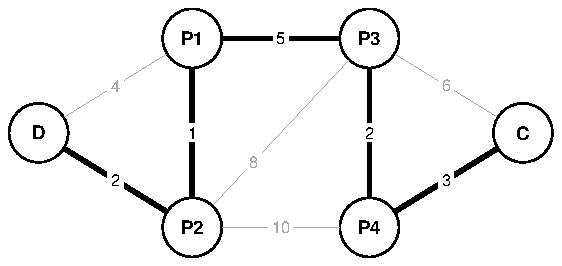
\includegraphics[width=0.75\textwidth]{imagens/grafo-coleta.pdf}
  \caption*{Fonte: Elaborada pela autora (2027).}
\end{figure}

A legenda vem acima da figura, com número, travessão e título, e a fonte vem
abaixo, mesmo quando a figura é da própria autora (Manual, p. 16-17).

Para aplicar os métodos do Capítulo~\ref{cap:metodos}, a tese vai precisar
dos seguintes dados de cada setor:

\begin{enumerate}
  \item a malha viária, com o comprimento e o sentido de cada trecho de rua;
  \item a localização dos pontos de coleta, da garagem e da cooperativa;
  \item para cada ponto:
  \begin{enumerate}
    \item a janela de atendimento, $[a_i, b_i]$;
    \item o tempo de serviço, $s_i$;
  \end{enumerate}
  \item as rotas praticadas hoje, para comparação.
\end{enumerate}

A lista tem subalíneas, que a classe marca com travessão (Manual, p. 71).

%==============================================================================
\chapter{Considerações finais}
\label{cap:consideracoes}
%==============================================================================

A revisão mostrou que a coleta seletiva com horários de atendimento cabe no
problema de roteamento de veículos com janelas de tempo, e que o algoritmo de
Dijkstra continua útil como primeira etapa, no cálculo das distâncias. Para
setores com poucas dezenas de pontos, uma heurística de inserção seguida de
busca local parece o ponto de partida mais simples, com a formulação exata
como referência nos setores menores. O próximo passo é levantar os dados do
Capítulo~\ref{cap:aplicacao} com a equipe de coleta.

%------------------------------------------------------------------------------
% Referências: estilo abnt.bst e base bibliografia.bib, ambos na raiz. Só as
% obras citadas no texto entram na lista.
%------------------------------------------------------------------------------
\bibliographystyle{abnt}
\bibliography{bibliografia}

%------------------------------------------------------------------------------
% Apêndices: material elaborado pela própria autora (Manual, p. 23).
% Anexos (\anexos) seguem a mesma lógica, para material de outra autoria; veja
% o exemplo de dissertação.
%------------------------------------------------------------------------------
\apendices

\chapter{Dados do grafo de exemplo}
\label{apx:dados}

O grafo da Figura~\ref{fig:grafo} tem seis vértices e nove arestas, com as
distâncias em quilômetros: D--P1, 4; D--P2, 2; P1--P2, 1; P1--P3, 5; P2--P3,
8; P2--P4, 10; P3--P4, 2; P3--C, 6; P4--C, 3. A rota mínima de D até C passa
por P2, P1, P3 e P4 e tem 13~km.

\end{document}
